
\section{TX Multiplexer}
The Transmit Multiplexer selects one of the six inputs for exclusive
access to the NIC output on a prioritized basis. The device connected
to port 0 has greatest priority. The armed status of port 1 is only
queried when port 0 is in an unarmed state. Thus it is possible, via
repeated arming of the input, for the device on port 0 to monopolize
access to the NIC.

In practice, with the Event Transmitter connected to Port 0, this
device will only have exclusive access for at most 550 clock ticks,
leaving almost half of the event cycle for data packet transmission
and other tasks.


\subsection{Interface}
The TX input mux selects among armed inputs. To send a packet, a
device asserts the \signal{ARM} signal and waits for the assertion of
the corresponding \signal{GRANT}.

Note that \signal{ARM} should be deasserted by the source once
\signal{GRANT} has been asserted to prevent multiple-triggering.

When \signal{GRANT} is asserted, that port is given the exclusive
control of the output to the NIC. The \signal{DEN} and and
\signal{DIN[15:0]} are passed through with one-cycle latency.

The transition of \signal{DEN} from high to low on a given port
indicates the completion of that port's transmission needs. To ensure a sufficient inter-frame space, a six-tick wait cycle is entered. After that, the
multiplexer will then query the \signal{ARM} status of the next device.


\subsection{Implementation}

When DENMUX transitions from high-to-low, that port has completed
sending its packet. Then, we deassert ARM and move on. \signal{ARM[n]}
arms the interface for a given port, and a priority decoder is used by
the FSM to determine the next interface to transmit via the setting of
\signal{LCHAN}.

\begin{figure}
\begin{centering}
\includegraphics[scale=0.8]{txmux.svg}
\end{centering}
\caption{FSM Transmit Multiplexer internal implementation.}
\label{txmux}
\end{figure}

\begin{figure}
\begin{centering}
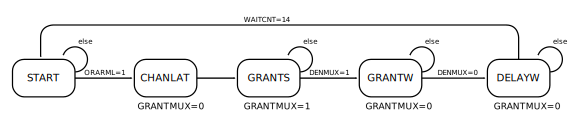
\includegraphics[scale=0.8]{txmux.fsm.svg}
\end{centering}
\caption{Transmit Multiplexer FSM. }
\label{txmux.fsm}
\end{figure}


